\documentclass[11pt]{article}

%----------------------------------------------------------------------
% Packages
%----------------------------------------------------------------------
\usepackage[margin=1in]{geometry}
\usepackage{amsmath, amssymb, amsthm}
\usepackage{mathtools}
\usepackage{bm}
\usepackage{graphicx}
\usepackage{hyperref}
\usepackage{xcolor}
\usepackage{booktabs}
\usepackage{enumitem}
\usepackage{microtype}
\usepackage[round,authoryear]{natbib}
\usepackage{tikz}
\usetikzlibrary{positioning, arrows.meta, calc}
\usepackage{bbm}

\hypersetup{
  colorlinks=true,
  linkcolor=blue!60!black,
  citecolor=blue!50!black,
  urlcolor=blue!60!black
}

%----------------------------------------------------------------------
% Theorem-like environments
%----------------------------------------------------------------------
\newtheorem{definition}{Definition}
\newtheorem{theorem}{Theorem}
\newtheorem{lemma}[theorem]{Lemma}
\newtheorem{proposition}[theorem]{Proposition}
\newtheorem{corollary}[theorem]{Corollary}
\newtheorem*{remark}{Remark}

%----------------------------------------------------------------------
% Macros
%----------------------------------------------------------------------
\newcommand{\R}{\mathbb{R}}
\newcommand{\E}{\mathbb{E}}
\renewcommand{\Pr}{\mathbb{P}}
\newcommand{\N}{\mathcal{N}}
\newcommand{\D}{\mathcal{D}}
\newcommand{\A}{\mathcal{A}}
\newcommand{\M}{\mathcal{M}}
\newcommand{\I}{\mathcal{I}}
\newcommand{\eps}{\varepsilon}
\newcommand{\sigm}{\sigma}
\newcommand{\dset}{D}
\newcommand{\dsetp}{D'}
\newcommand{\norm}[1]{\left\lVert #1 \right\rVert}
\newcommand{\abs}[1]{\left\lvert #1 \right\rvert}
\newcommand{\inner}[2]{\langle #1, #2 \rangle}
\newcommand{\clip}{\mathrm{clip}}
\newcommand{\sign}{\mathrm{sign}}
\newcommand{\relu}{\mathrm{ReLU}}
\newcommand{\softmax}{\mathrm{softmax}}
\newcommand{\LN}{\mathrm{LN}}
\newcommand{\divyam}[1]{\textcolor{red}{Divyam: }\textcolor{red}{#1}}

\title{Privacy Backdoors and the Tightness of DP-SGD}
\author{Divyam Anshumaan, Ronak Chauhan, Sarthak Choudhary
}
\date{\today}


\begin{document}
\maketitle

\begin{abstract}
Abstract goes here ....
\end{abstract}

%----------------------------------------------------------------------
\section{Introduction}

Sharing and fine-tuning pretrained models has become a default practice in modern machine learning. Public repositories such as Hugging Face host hundreds of thousands of models, and practitioners routinely download these weights, attach a fresh classification head, and fine-tune on their own data. The datasets used for fine-tuning frequently contain sensitive information, such as medical records, user conversations, or internal communications. It is therefore standard practice to analyze the privacy properties of the resulting model and, increasingly, to adopt differentially private training procedures such as DP-SGD~\citep{abadi2016deep}. 

Two independent classes of risk have been studied in the fine-tuning pipeline. The first is a \textbf{supply-chain} risk that stems from the source of the pretrained weights: a malicious provider can tamper with a model's weights so that it misbehaves on specific inputs, compromising the model's \emph{integrity}~\citep{gu2017badnets, liu2018trojaning, hong2022handcrafted}. The second is a \textbf{memorization} risk that stems from the training procedure itself: neural networks trained (or fine-tuned) on sensitive data encode non-trivial information about individual examples, enabling membership inference~\citep{shokri2017membership} and data extraction~\citep{carlini2021extracting}. DP-SGD is the canonical defense against the second risk, bounding the per-example influence of the final weights, and is typically deployed under the implicit assumption that the initialization is benign. \\

\paragraph{Privacy backdoors.} \citet{feng2024privacy} introduce \emph{privacy backdoors}, which bridge the integrity and privacy threats described above. They show that a malicious provider can tamper with a pretrained model's weights so that, during ordinary fine-tuning on the victim's private dataset, individual training examples are imprinted into the weights in a form that the attacker can later recover. The construction relies on a novel primitive, which the authors term a \emph{data trap}: a small number of units are configured so that the gradient update induced by a specific training example is written with high fidelity into an attacker-chosen set of coordinates, and so that no subsequent update overwrites the signal. An adversary with access only to the final fine-tuned model can then read off the captured example directly from those coordinates.

\paragraph{Implications for DP-SGD.} The most consequential aspect of the attack is arguably not the reconstruction of the individual examples but its bearing on \emph{differential privacy}. The privacy analysis of DP-SGD rests on a worst-case condition: the per-example gradient differs maximally, on some coordinate, between the neighboring datasets~\citep{abadi2016deep}. The induced per-step bound is tight for the Gaussian mechanism; its composition across training steps, however, is widely believed to be pessimistic in practice, as the corresponding adversary is assumed to observe intermediate noisy gradient~\citep{nasr2021adversary}. In contrast, a realistic \emph{end-to-end} adversary, with access only to the deployed fine-tuned model, is expected to extract substantially less information than this bound permits; an intuition that has motivated the use of comparatively loose privacy budgets in the production deployments (e.g., $\varepsilon \geq 8$, or $\varepsilon \approx 9$ in \citet{ramaswamy2020training}).

Privacy backdoors invalidate this intuition. The data-trap primitive can be specialized so that, at every DP-SGD step, the gradient of the target example concentrates entirely on a small, attacker-known index set, with $\ell_2$-norm equal to the clipping threshold, while the gradients of all other examples vanish on that set. This constitutes precisely the per-step worst case assumed by the analysis. \citet{feng2024privacy} shows analytically that, under this construction, an end-to-end adversary observing only the final weights can derive a lower bound on the realized $\varepsilon$ that closely matches the provable upper bound. The discrepancy between the theoretical and empirical privacy of end-to-end DP-SGD is thus not attributable to structural slack in the analysis; it is a consequence of  benign initializations and disappears under an adversarial one.

\paragraph{Scope.} This report provides a self-contained exposition of \citet{feng2024privacy}, organized around two questions.
\begin{enumerate}[label=(\roman*), leftmargin=*, itemsep=2pt, topsep=2pt]
  \item \textbf{Construction.} How can an adversary engineer a pretrained initialization whose weights capture individual fine-tuning examples and preserve the captured signal across many SGD steps with gradient clipping and Gaussian noise?
  \item \textbf{Tightness.} Why does such an adversarial initialization render the end-to-end privacy leakage of DP-SGD nearly tight against its provable upper bound, and what is the resulting closed-form lower bound on the realized $\eps$?
\end{enumerate}


\section{Problem Statement}
\label{sec:problem}

This section formalizes the setting in which privacy backdoors operate. We describe the fine-tuning pipeline and fix notation (Section~\ref{sec:setup}), specify the adversary's capabilities and the victim's training procedure (Section~\ref{sec:threat}), and state the adversary's formal objectives (Section~\ref{sec:goal}).

\subsection{Setup}
\label{sec:setup}

We consider the standard fine-tuning pipeline for supervised classification. A model provider publishes a pretrained backbone $\theta_0^{\mathrm{bb}} \in \mathbb{R}^{d_{\mathrm{bb}}}$. A victim downloads these weights, appends a freshly initialized classification head $\theta_0^{\mathrm{head}} \in \mathbb{R}^{d_{\mathrm{head}}}$ drawn from a standard initializer, and forms the initial parameter vector $\theta_0 \coloneqq (\theta_0^{\mathrm{bb}}, \theta_0^{\mathrm{head}}) \in \mathbb{R}^d$ with $d = d_{\mathrm{bb}} + d_{\mathrm{head}}$. The victim then fine-tunes on a private dataset $\dset = \{(x_i, y_i)\}_{i=1}^{n} \subset \mathcal{X} \times \mathcal{Y}$, where $\mathcal{X}$ denotes the input space and $\mathcal{Y} = \{1, \ldots, C\}$ is the label space of $C$-way classification task. Fine-tuning is performed by a training algorithm $\A$, producing the fine-tuned weights $\theta_T = \A(\theta_0, \dset)$. The adversary in our setting is the model provider itself: having controlled the backbone coordinates of $\theta_0$, it subsequently obtains access to $\theta_T$.

\subsection{Threat Model}
\label{sec:threat}

\paragraph{Adversary.} The adversary fully controls the pretrained backbone $\theta_0^{\mathrm{bb}}$, subject only to a utility constraint: the fine-tuned model must remain sufficiently accurate on the downstream task that the victim accepts and deploys it. The adversary does not participate in the fine-tuning process and observes no intermediate state of the run, i.e., no per-step gradients. Its only interaction with the fine-tuning pipeline is through the final model $\theta_T$ produced by the victim.


\paragraph{Victim.} The victim performs standard supervised fine-tuning on the private dataset $\dset$ using a fixed training algorithm $\A$. We consider two instantiations of $\A$, corresponding to the non-private and differentially private regimes:

\begin{itemize}[leftmargin=*, itemsep=2pt, topsep=2pt]
    \item \emph{Full fine-tuning with SGD.} All coordinates of $\theta_0$ are updated via mini-batch stochastic gradient descent for $T$ steps. This is the setting of the reconstruction attack of Section~\ref{sec:attack}.
    \item \emph{Top-$k$ fine-tuning with DP-SGD.} The bottom portion of the backbone is frozen, and only the top $k$ layers together with the classification head are updated, using the DP-SGD algorithm of ~\citet{abadi2016deep}. This is the standard setup for differentially private transfer learning \citep{tramer2020differentially}, and is the setting under which the tightness of consequence of Section~\ref{sec:privacy} is established.
\end{itemize}

In both regimes, fine-tuning is carried out end-to-end by the victim, without any adversarial participation.

\paragraph{Access to the fine-tuned model.}
We restrict attention to the \emph{white-box} setting, in which the adversary reads the fine-tuned parameter vector $\theta_T$ directly. This models a fine-tuned model that is redistributed internally or externally, or one whose weights are otherwise recovered by the adversary after deployment. We note in passing that the attack admits a black-box extension in which the adversary only queries the  deployed model on inputs of its choice; the black-box setting is not pursued in this report.

\subsection{Objective}
\label{sec:goal}

The adversary's objective has two components: a privacy compromise, formalized as the ability to reconstruct individual fine-tuning examples from the released model; and a utility constraint, formalized as a bound on the degradation of the downstream task performance relative to a benign pretrained initialization.

For the reconstruction goal, we assume the input space $\mathcal{X}$ is equipped with a dissimilarity measure $\rho: \mathcal{X} \times \mathcal{X} \to \mathbb{R}_{\geq 0}$ (for instance, the Euclidean distance on normalized images, or a token-level edit distance on text). Let $\mathcal{P}$ denote a distribution over datasets of size $n$ in $\mathcal{X} \times \mathcal{Y}$, from which the victim draws the private dataset $\dset$.

\begin{definition}[Reconstruction]
    \label{def:recon}
    A pair $(\theta_0, \mathrm{Ext})$, consisting of an initialization $\theta_0 \in \mathbb{R}^d$ and a (possibly randomized) extraction algorithm $\mathrm{Ext}: \mathbb{R}^d \to \mathcal{X}^{\ast}$, achieves \emph{$(k, \tau, \beta)$-reconstruction} under the training algorithm $\A$ and dataset distribution $\mathcal{P}$ if 
    \[
      \Pr\!\left[\,\left|\left\{\, (x, y) \in \dset \;:\; \min_{\hat{x} \in \mathrm{Ext}(\theta_T)} \rho(x, \hat{x}) \,\leq\, \tau \,\right\}\right| \,\geq\, k \,\right] \;\geq\; 1 - \beta,
    \]
    where $\dset \sim \mathcal{P}$, $\theta_T = \A(\theta_0, \dset)$, and the probability is taken over the randomness of $\dset$,  $\A$, and $\mathrm{Ext}$.
\end{definition}


\begin{definition} [Utility preservation]
\label{def:util}
    Let $\theta_0^{\mathrm{ref}}$ be a benign reference initialization (with a clean pretrained backbone). For a parameter vector $\theta \in \mathbb{R}^d$ and a dataset $D' \subset \mathcal{X} \times \mathcal{Y}$, let 
    \[
        \mathrm{Acc}(\theta; \dset') \;\coloneqq\; \frac{1}{|\dset'|} \sum_{(x, y) \,\in\, \dset'} \mathbbm{1}\!\left[\, f_\theta(x) = y \,\right]
    \]
    denote the empirical accuracy of the classifier $f_\theta: \mathcal{X} \to \mathcal{Y}$ on $D'$. initialization $\theta_0$ is \emph{$\gamma$-utility-preserving relative to $\theta_0^{\mathrm{ref}}$} under the training algorithm $\A$ and distribution $\mathcal{P}$ if 
    \[
      \E\!\left[\,\mathrm{Acc}\!\left(\A(\theta_0^{\mathrm{ref}}, \dset); \dset \right) \,-\, \mathrm{Acc}\!\Big(\A(\theta_0, \dset); \dset\Big)\right] \;\leq\; \gamma,
    \]
    where the expectation is taken over the randomness of $D$ and $\A$.
\end{definition}

A successful privacy backdoor is an initialization $\theta_0$ paired with an extraction algorithm $\mathrm{Ext}$ that meets both objectives simultaneously: the pair achieves $(k, \tau, \beta)$-reconstruction in the sense of Definition~\ref{def:recon} for small $\tau$ and $\beta$, while $\theta_0$ is $\gamma$-utility-preserving in the sense of Definition~\ref{def:util} for small $\gamma$.

\paragraph{A consequence for DP-SGD.} Definitions~\ref{def:recon} and~\ref{def:util} make no reference to differential privacy. When $\A$ is DP-SGD, however, a successful privacy backdoor yields, as a byproduct, an analytic lower bound on the realized privacy parameter $\varepsilon$. This lower bound is a consequence of the reconstruction objective, and we defer its statement and proof to Section~\ref{sec:privacy}.
\section{Backdooring MLPs for White-box Data Stealing}
\label{sec:attack}
The goal of the adversary is to have the privacy backdoor capture exactly one finetuning data point. In a federated learning setting, the attacker gets to see gradient updates directly, making it feasible to determine finetuning data points. However, in this setting, the adversary only receives the finetuned model \textit{after} the entire training run is complete. Therefore, the backdoor must be engineered in such a way that the captured inputs: 
\begin{enumerate}[label=(\roman*), leftmargin=*, itemsep=2pt, topsep=2pt]
    \item can be extracted from the weights of the finetuned model,
    \item ``survive'' the entire training run, without being mixed up with other inputs captured in subsequent training steps.
\end{enumerate}

To accomplish both criteria, the authors propose \textit{data trap}, a backdoor with a ``single-use'' property; once the backdoor has been activated, it will never be active again afterwards.

\subsection{Data Traps}
We illustrate the approach by backdooring a single linear unit (i.e., one element of a linear layer) and then work our way to a full MLP. Let $\mathbf{w} \in \mathbb{R}^m$ and $b \in \mathbb{R}$ be the weights and bias of the unit. Suppose $\mathbf{x}\in \mathbb{R}^m$ is the input of the unit. We define the unit's activation $h$ as, 
\begin{equation}
    h = \mathtt{ReLU}\big(\mathbf{w}^\top\mathbf{x} + b \big)
\end{equation}

As described in~\cite{fowl2022robbingfeddirectlyobtaining}, the parameters $\mathbf{w}$ and $b$ can be set to ensure that, with high probability, a single input $\mathbf{x}$ in a training batch activates the neuron (i.e. $h > 0$). When the weights update by backpropagating the training loss $\mathcal{L}$, we then get:
\begin{align}
    \nabla_\mathbf{w} \mathcal{L} = \frac{\partial \mathcal{L}}{\partial h} \cdot \mathbf{x}, \qquad \nabla_b \mathcal{L} = \frac{\partial \mathcal{L}}{\partial h}.
\end{align}

\paragraph{Recovering data.} We update the weights and bias of the unit as:
\begin{align}
    \mathbf{w}' \gets \mathbf{w} - \eta \cdot \nabla_\mathbf{w} \mathcal{L}, \qquad b' \gets b - \eta \cdot\nabla_b \mathcal{L}.
\end{align}

Knowledge of the learning rate, the original weights and bias allows us to recover $\nabla_\mathbf{w} \mathcal{L}$ and $\nabla_b \mathcal{L}$. Dividing $\nabla_\mathbf{w} \mathcal{L}$ by $\nabla_b \mathcal{L}$ recovers $\mathbf{x}$.

\paragraph{Preventing subsequent updates.} We now need to ensure that the gradient update for $\mathbf{x}$ closes the backdoor, i.e., prevents further updates. Assume that the backdoor activates on input $\hat{\mathbf{x}}$. The updated backdoor's output on a new input $\mathbf{x}$ is:
\begin{align}
    h' &= \mathtt{ReLU}\big(\mathbf{w}'^\top \mathbf{x} + b'\big) \\&= \mathtt{ReLU}\big[(\mathbf{w}^\top \mathbf{x} + b) - \eta \cdot \frac{\partial L}{\partial h} \cdot \left( \hat{\mathbf{x}}^\top \mathbf{x} + 1 \right)\big]
\end{align}


For the $\mathtt{ReLU}$ activation function, a sufficient condition for the backdoor to close (i.e. $h' = 0$ for all $\mathbf{x}$, so all subsequent $\frac{\partial h'}{\partial x} = 0$) is to ensure $\mathbf{w}'^\top\mathbf{x} + b' \leq 0$. This is achieved by:

\begin{enumerate}[label=(\roman*), leftmargin=*, itemsep=2pt, topsep=2pt]
    \item $\hat{\mathbf{x}}^\top \mathbf{x} + 1 > 0$,
    \item $\frac{\partial L}{\partial h}$ is sufficiently large and positive.
\end{enumerate}

The first condition $\hat{\mathbf{x}}^\top \mathbf{x} + 1 > 0$ only depends on the input, and can be algorithmically enforced (e.g., by mapping inputs to $[0,1]^m$, which ensures all dot products are non-negative). We take a closer look at the second condition in the following subsection.

\subsubsection{Ensuring a large, positive gradient.} 

\begin{figure}[t]
\centering
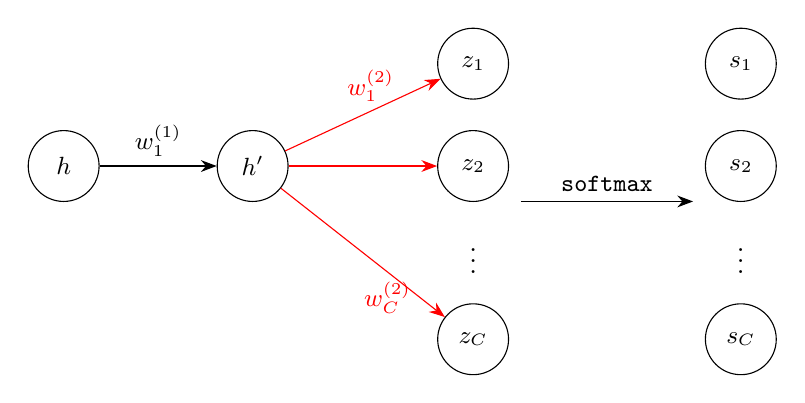
\begin{tikzpicture}[
    >={Stealth[length=2mm]},
    node/.style={circle, draw, minimum size=0.9cm, inner sep=0pt, font=\small},
    every label/.style={font=\small}
]
    % Input nodes h and h'
    \node[node] (h)  at (0, 0)    {$h$};
    \node[node] (hp) at (2.4, 0)  {$h'$};

    % Logits z_1, z_2, ..., z_C
    \node[node] (z1) at (5.2,  1.3) {$z_1$};
    \node[node] (z2) at (5.2,  0)   {$z_2$};
    \node       (zd) at (5.2, -1.1) {$\vdots$};
    \node[node] (zC) at (5.2, -2.2) {$z_C$};

    % Softmax outputs s_1, s_2, ..., s_C
    \node[node] (s1) at (8.6,  1.3) {$s_1$};
    \node[node] (s2) at (8.6,  0)   {$s_2$};
    \node       (sd) at (8.6, -1.1) {$\vdots$};
    \node[node] (sC) at (8.6, -2.2) {$s_C$};

    % Black edge: h -> h'
    \draw[->] (h) -- node[above, font=\small] {$w_1^{(1)}$} (hp);

    % Red edges: h' -> z_i (classification head)
    \draw[->, red] (hp) -- node[above, pos=0.55, font=\small] {$w_1^{(2)}$} (z1);
    \draw[->, red] (hp) -- (z2);
    \draw[->, red] (hp) -- node[below, pos=0.65, font=\small] {$w_C^{(2)}$} (zC);

    % Softmax arrow from logits block to softmax block
    \draw[->] ($(z1.east)!0.5!(zC.east) + (0.15,0)$)
        -- node[above, font=\ttfamily\small] {softmax}
        ($(s1.west)!0.5!(sC.west) - (0.15,0)$);
\end{tikzpicture}
\caption{Illustration of the output of a data trap
($h = \mathtt{ReLU}\!\left(\mathbf{w}^\top \mathbf{x} + b\right)$)
connected to the model's output. The weights of the classification head
(in red) are typically not under the control of the attacker, and
randomly initialized before finetuning.}
\label{fig:datatrap}
\end{figure}

Suppose the new finetuing linear layer is $\mathbf{w}^{(2)} = (w^{(2)}_1,\dots, w^{(2)}_C)$, where $C$ are the number of classes for the finetuning task. It is added in front of the last layer of the pretrained model, as shown in Figure~\ref{fig:datatrap}.  We connect the backdoor output $h$ to a hidden unit $h'$ with weight $w^{(1)}_1$, i.e.,
\[
    h' = \mathtt{ReLU}\!\left(w^{(1)}_1h\right).
\]

The unit $h'$ is then connected via the new linear layer $\mathbf{w}^{(2)}$ to the model's logit layer $\mathbf{z}$. The logits are passed through a softmax before computing the cross-entropy loss (for some target class $T$). Starting from the backdoor, the computation proceeds as follows:

\begin{enumerate}
    \item Hidden unit activation: $h' = \mathtt{ReLU}\!\left(w^{(1)}_1h\right)$ Note that $h > 0$ by construction.
    \item Logits: $z_i =w^{(2)}_i h'$ for each class $i \in \{1,\dots,C\}$
    \item Softmax: $s_i = \exp(z_i)/\sum^C_{j=1}\exp(z_j)$
    \item Cross-entropy loss: $\mathcal{L} = -\sum^C_{i=1}y_i\log(s_i)$, where $y_i = \begin{cases} 1 & \text{if } i = T, \\ 0 & \text{otherwise.} \end{cases}
$.
\end{enumerate}

A standard gradient calculation gives:
\begin{align}
    \frac{\partial \mathcal{L}}{\partial h} = \frac{\partial \mathcal{L}}{\partial h'} \cdot \frac{\partial h'}{\partial h} = \left( \sum_{i=1}^{C} (s_i - y_i) \cdot w_i^{(2)} \right) \cdot w_1^{(1)}
\end{align}

Taking into account the values of $y_i$, this can be expressed as: 

\begin{align}
\label{eq:gradient}
    \frac{\partial \mathcal{L}}{\partial h} = \left( \sum_{i=1}^{C} \Big(s_i \cdot w_i^{(2)}\Big) - w_T^{(2)} \right) \cdot w_1^{(1)}
\end{align}

In order to ensure $\frac{\partial \mathcal{L}}{\partial h}$ is large, we set $w_1^{(1)}$ to be a large value. Now let's analyze the implications of a large $w_1^{(1)}$. Consider $s_i$:

\[
s_i = \frac{\exp(z_i)}{\sum^C_{j=1}\exp(z_j)} =  \frac{\exp(w^{(2)}_i h')}{\sum^C_{j=1}\exp(w^{(2)}_j h')}
\]

Factorizing $\exp(w^{(2)}_i h')$, we get:
\begin{align}
\label{eqn:neg-diff}
    s_i = \frac{1}{1 + \sum^C_{j\neq i}\exp\big((w^{(2)}_j - w^{(2)}_i) h'\big)}
\end{align}

Since $\mathbf{w}^{(2)}$ is randomly initialized, there exists $w^{(2)}_k = \max \{w^{(2)}_1,\dots, w^{(2)}_C\}$ (ignoring ties). However, $h' = \mathtt{ReLU}\!\left(w^{(1)}_1h\right)$ is a large and positive value, since $w^{(1)}_1$ is large and positive, with $h > 0$. Then,

\paragraph{Case 1: $i = k$.} Since $w^{(2)}_k$ is the largest value in $\mathbf{w}^{(2)}$, $(w^{(2)}_j - w^{(2)}_i) < 0$ for all $j\neq i$ in  Eq.~\eqref{eqn:neg-diff}. Then for all $j\neq i$, $\exp\!\big((w^{(2)}_j - w^{(2)}_i)\, h'\big) \approx 0$. Therefore, 

\[
    \sum^C_{j\neq i}\exp\big((w^{(2)}_j - w^{(2)}_i) h'\big) \approx0
\]

\paragraph{Case 2: $i \neq k$.} There will be at least one term $(w^{(2)}_j - w^{(2)}_i) > 0$, where $j = k$. Then for that term, $\exp\!\big((w^{(2)}_j - w^{(2)}_i)\, h'\big) \approx \inf$. Therefore,

\[
    \sum^C_{j\neq i}\exp\big((w^{(2)}_j - w^{(2)}_i) h'\big) \approx \inf
\]

Substituting these cases in Eq.~\eqref{eqn:neg-diff}, we get:
\[
s_i \approx 
\begin{cases} 1 & \text{if } i = k, \\ 0 & \text{if } i \neq k. \end{cases}
\]

Using this knowledge in Eq.~\eqref{eq:gradient}, we find that:
\begin{align}
\label{eq:reveal}
    \frac{\partial \mathcal{L}}{\partial h} &= \left( \sum_{i=1}^{C} \Big(s_i \cdot w_i^{(2)}\Big) - w_T^{(2)} \right) \cdot w_1^{(1)}\\
    & \approx \big(w^{(2)}_k - w_T^{(2)}\big) \cdot w_1^{(1)}
\end{align}

8Now, whenever $T\neq k$, i.e., the target class does not correspond to the largest weight in the linear layer, $\frac{\partial \mathcal{L}}{\partial h} > 0$. The probability of $T = k$ is $1/C$, (as $k \in \{1, \dots C\}$). Therefore, a sufficiently large $w_1^{(1)}$ also guarantees that $\frac{\partial \mathcal{L}}{\partial h}$ is positive with probability $1 - 1/C$. This closes the backdoor and prevents subsequent updates from corrupting the captured inputs.
\section{Privacy Analysis}
\label{sec:privacy}

This section establishes the central claim of the report: under a privacy backdoor, the end-to-end privacy analysis of DP-SGD is nearly tight. We first recall DP-SGD and its upper bound, then develop a hypothesis-testing lower bound on $\varepsilon$ that applies to any mechanism, and finally instantiate this lower bound under the backdoor construction of Section~\ref{sec:attack} to show that it matches the upper bound.

\subsection{DP-SGD and its privacy upper bound}
\label{sec:dpsgd}

Fix a per-example loss $\ell$. DP-SGD \citep{abadi2016deep} iterates, for $t=1, \ldots, T$:
\begin{enumerate}[label=(\roman*), leftmargin=*, itemsep=2pt, topsep=2pt]
  \item Sample a lot $S_t \subseteq [n]$ by Poisson subsampling with rate
    $q = L/n$;
  \item Compute per-example gradients and clip to norm $C$:
    $g_t(i) = \clip_C\!\left(\nabla_\theta \ell(\theta_{t-1}; x_i, y_i)\right)$
    for each $i \in S_t$;
  \item Form the noisy aggregate
    $G_t = \sum_{i \in S_t} g_t(i) + \xi_t$, where
    $\xi_t \sim \mathcal{N}(0, \sigm^2 C^2 I_d)$;
  \item Update $\theta_t = \theta_{t-1} - (\eta/L)\, G_t$.
\end{enumerate}

\begin{theorem}[DP-SGD privacy upper bound; \citealp{abadi2016deep,
mironov2019r}]
\label{thm:upper}
For any $\delta \in (0, 1)$, there exists $\eps^\star(\sigm, q, T, \delta)$, computable from the subsampled-Gaussian R\'enyi-DP accountant,
such that the map $\dset \mapsto (G_1, \ldots, G_T)$ is $(\eps^\star,
\delta)$-differentially private.
\end{theorem}

Because $\theta_T$ is a deterministic function of $\theta_0$ and $(G_1, \ldots, G_T)$, the post-processing theorem of DP \citep{dwork2014algorithmic} implies that end-to-end map $\dset \mapsto \theta_T$ is also $(\eps^\star, \delta)$-DP. \textbf{The question is whether this upper bound is tight when the adversary sees only $\theta_T$.}

\subsection{End-to-end versus per-step adversaries}
\label{sec:endtoend}

Two adversary models inherit the upper bound $\eps^\star$ via post-processing. A \emph{per-step} adversary observes the full trajectory $(G_1, \ldots, G_T)$; an \emph{end-to-end} adversary observes only $\theta_T$. Empirical auditing shows that $\eps^\star$ is essentially tight in the per-step regime, but audits of end-to-end DP-SGD from benign initializations typically saturate at $\tilde\eps \approx \eps^\star / 4$ or less \citep{nasr2021adversary, jagielski2020auditing}. This apparent slack is often cited in support of loose production privacy budgets, e.g.\ $\eps \in [8,9]$ \citep{ramaswamy2020training}. Whether it reflects structural slack in the analysis, or merely the benign initialization assumed by existing audits, is the question we answer.

\subsection{Privacy as hypothesis testing}
\label{sec:ht-dp}

We first record the reduction from differential privacy to a hypothesis-testing constraint. The reduction is mechanism-agnostic and will be applied to DP-SGD in Section~\ref{sec:instantiation}.


Let $M : \mathbb{D} \to \Delta(\mathcal{R})$ be a randomized mechanism mapping datasets to distributions over an output space $\mathcal{R}$. Two datasets $D_0, D_1 \in \mathbb{D}$ are \emph{neighbors}, written $D_0 \sim D_1$, if they differ by a single record. In the membership-inference specialization to which we will reduce, $D_1 = D \cup \{x^\star\}$ and $D_0 = D$ for a target canary $x^\star$, and the adversary must decide from $Y \sim M(D_b)$ whether $b = 0$ or $b = 1$.

\begin{definition}[Deterministic test]
\label{def:det-test}
A \emph{test} is specified by a measurable rejection region $R \subseteq \mathcal{R}$: the adversary declares ``$x^\star$ present'' if $Y \in R$ and ``$x^\star$ absent'' otherwise. Its power is summarized by
\[
  \mathrm{TPR}(R) = \Pr_{Y \sim M(D_1)}[Y \in R],
  \qquad
  \mathrm{FPR}(R) = \Pr_{Y \sim M(D_0)}[Y \in R].
\]
\end{definition}

\begin{lemma}[Hypothesis-testing constraint]
\label{lem:tpr-fpr}
If $M$ is $(\eps, \delta)$-differentially private, then for every rejection region $R \subseteq \mathcal{R}$,
\[
  \mathrm{TPR}(R) \;\leq\; e^\eps \cdot \mathrm{FPR}(R) + \delta.
\]
\end{lemma}

\begin{proof}
Apply the definition of $(\eps, \delta)$-DP with measurable set $S = R$ to the neighboring pair $D_0 \sim D_1$ and substitute the definitions of $\mathrm{TPR}$ and $\mathrm{FPR}$.
\end{proof}

\begin{proposition}[Hypothesis-testing lower bound on $\eps$]
\label{prop:eps-lb}
For every rejection region $R$ with $\mathrm{FPR}(R) > 0$,
\begin{equation}
  \eps \;\geq\; \log\!\left(\frac{\mathrm{TPR}(R) - \delta}{\mathrm{FPR}}\right).
  \label{eq:eps-lb-pointwise}
\end{equation}
Consequently, if one defines
\[
  \tilde\eps(M, \delta) \;\coloneqq\; \sup_{R \subseteq \mathcal{R}}
  \log\!\left(\frac{\mathrm{TPR}(R) - \delta}{\mathrm{FPR}(R)}\right),
\]
then any valid $(\eps, \delta)$-DP guarantee for $M$ must satisfy $\eps \geq \tilde\eps(M, \delta)$.
\end{proposition}

\begin{proof}
Rearrange Lemma~\ref{lem:tpr-fpr} and take the supremum over $R$.
\end{proof}

\subsection{Reduction to a scalar threshold test}
\label{sec:threshold}

Optimizing $\tilde\eps$ over $R \subseteq \mathcal{R}$ is intractable for $\mathcal{R} = \R^d$. The standard simplification is to project the output through a scalar test statistic and restrict attention to threshold rejection regions.

\begin{definition}[Threshold test]
\label{def:thr-test}
Given a measurable test statistic $\Delta : \mathcal{R} \to \R$, the \emph{threshold family} is $\{R_t\}_{t \in \R}$ with $R_t = \{y \in \mathcal{R} : \Delta(y) \geq t\}$. Define
\[
  \tilde\eps_{\mathrm{thr}}(\Delta, \delta)
  \;\coloneqq\; \sup_{t \in \R}
  \log\!\left(\frac{\Pr_{Y \sim M(D_1)}[\Delta(Y) \geq t] - \delta}
                     {\Pr_{Y \sim M(D_0)}[\Delta(Y) \geq t]}\right).
\]
\end{definition}

By the Neyman--Pearson lemma, if $\Delta$ is a monotone function of the log-likelihood ratio $\Lambda(y) = \log \frac{dM(D_1)}{dM(D_0)}(y)$, then threshold tests on $\Delta$ are uniformly most powerful: for every $\alpha \in [0, 1]$ there is a $t$ such that $R_t$ maximizes $\mathrm{TPR}(R)$ subject to $\mathrm{FPR}(R) \leq \alpha$ among \emph{all} tests. In that case $\tilde\eps_{\mathrm{thr}}(\Delta, \delta) = \tilde\eps(M, \delta)$, i.e., no tightness is lost by restricting to threshold tests. When $\Lambda$ is not available in closed form, one may replace it with an approximation; the privacy backdoor construction of the next subsection is engineered so that a single coordinate of $\theta_T$ is, up to known affine shifts, a sufficient statistic for $\Lambda$, and the restriction is therefore without loss. The optimal threshold $t^\star$ is then found by grid search.

\subsection{Instantiation under a privacy backdoor}
\label{sec:instantiation}

We now instantiate Section~\ref{sec:threshold} on DP-SGD applied to a backdoored initialization. Fix a target canary $x^\star$ and consider the neighboring datasets $D_0 = \{(x_i, y_i)\}_{i=1}^{n-1}$ and $D_1 = D_0 \cup \{x^\star\}$. Let $\theta_T = \A_{\mathrm{DP\text{-}SGD}}(\theta_0, D_b)$.

\paragraph{The canary construction.} The construction of
Section~\ref{sec:attack} can be specialized to produce a canary \emph{module} rather than a single-use reconstruction trap: a configuration of the backbone weights, together with a known coordinate $j^\star$ and known affine shifts $(\alpha, \beta) \in \R \times \R_{>0}$, such that the clipped per-example gradient along $j^\star$ satisfies, for every step $t$,
\begin{equation}
  g_t(i)[j^\star] \;=\;
  \begin{cases}
    C & \text{if } i = x^\star \text{ and } x^\star \in S_t, \\
    0 & \text{otherwise}.
  \end{cases}
  \label{eq:canary-grad}
\end{equation}

Unlike the latched reconstruction trap of Section~\ref{sec:attack}, the canary module is \emph{multi-use}: \eqref{eq:canary-grad} holds at every step, not only at the first activation. The latch is unnecessary here because the canary does not encode an input-dependent payload; the attacker knows $x^\star$ a priori, so there is no information that needs to be preserved from being updated. The construction must instead secure two invariants: the clipped per-example gradient on coordinate $j^\star$ equals $\pm C$ when $i = x^\star$ is in the lot and $0$ otherwise, and the detector's activation condition on $x^\star$ is preserved across all $T$ steps.

Both invariants are produced by standard architectural choices. The trap unit is tuned so that it activates only for inputs in a small neighborhood of $x^\star$, which forces every $i \neq x^\star$ to contribute zero gradient through the amplifier path, including on coordinate $j^\star$. For $i = x^\star$, an amplifier gain $M \gg 1$ ensures that the pre-clip gradient $\nabla_\theta \ell(\theta_{t-1}; x^\star)$ is dominated by a term of magnitude $M$ along $e_{j^\star}$, so clipping by the factor $C/M$ yields $\pm C$ on coordinate $j^\star$ and $O(C/M)$ on every other coordinate. Because non-target examples leave the detector weights untouched, and the target's own contribution to those weights is $O(C/M)$ per step, the cumulative drift of any detector coordinate across $T$ steps is bounded by $O(\eta T C / (L M)) + O(\eta \sigma C \sqrt{T}/L)$, which is small by choice of $M$ relative to the activation margin with which the detector is configured. The detector, therefore, remains operational throughout training.

\paragraph{Scalar reduction.} Define the canary statistic
$\Delta(\theta) \coloneqq (\theta[j^\star] - \alpha) / \beta$. Under
DP-SGD, combining \eqref{eq:canary-grad} with the noise addition at
coordinate $j^\star$ gives
\begin{equation}
  \Delta(\theta_T) \;=\; \sum_{t=1}^T \big(C \cdot B_t + Z_t\big),
  \qquad
  Z_t \sim \mathcal{N}(0, \sigm^2 C^2) \text{ i.i.d.,}
  \label{eq:delta}
\end{equation}
where $B_t = \mathbbm{1}[x^\star \in S_t]$. Under $D_0$, the canary is
absent and $B_t \equiv 0$; under $D_1$, $B_t \stackrel{\mathrm{i.i.d.}}{\sim}
\mathrm{Bernoulli}(q)$. Writing $X_t \coloneqq C B_t + Z_t$, equation
\eqref{eq:delta} is the $T$-fold sum of i.i.d.\ copies of the
subsampled-Gaussian step \citep{mironov2019r}, and the induced
marginals are
\begin{align}
  \Delta(\theta_T) \,\big|\, D_0 &\;\sim\; \mathcal{N}(0, T \sigm^2 C^2),
  \label{eq:dist0} \\
  \Delta(\theta_T) \,\big|\, D_1 &\;\sim\; C \cdot \mathrm{Bin}(T, q)
  \,+\, \mathcal{N}(0, T \sigm^2 C^2), \label{eq:dist1}
\end{align}
where \eqref{eq:dist1} denotes the distribution of the sum of an
independent $C \cdot \mathrm{Bin}(T, q)$ draw and a Gaussian with
variance $T \sigm^2 C^2$.

\paragraph{Sufficiency and optimality.} The likelihood ratio between
\eqref{eq:dist1} and \eqref{eq:dist0} depends on $\theta_T$ only through
$\Delta(\theta_T)$, so $\Delta$ is a sufficient statistic for
distinguishing $D_0$ from $D_1$; moreover, the ratio is monotone
non-decreasing in $\Delta$. By Neyman--Pearson, threshold tests on
$\Delta$ are uniformly most powerful.
% and
% $\tilde\eps_{\mathrm{thr}}(\Delta, \delta) = \tilde\eps(M, \delta)$.

\paragraph{Main theorem.} The scalar mechanism defined by
\eqref{eq:delta} is, by construction, the subsampled Gaussian
mechanism with sampling rate $q$ and noise multiplier $\sigm$ iterated
$T$ times, whose optimal privacy curve is known
\citep{mironov2019r} to match the DP-SGD upper bound of
Theorem~\ref{thm:upper}. We therefore obtain:

\begin{theorem}[End-to-end tightness under a privacy backdoor]
\label{thm:main}
Let $\theta_0$ be the backdoored initialization of Section~\ref{sec:attack} with canary module \eqref{eq:canary-grad}. Let $\eps^\star(\sigm, q, T, \delta)$ be the DP-SGD upper bound of Theorem~\ref{thm:upper}, and let $\tilde\eps(\sigm, q, T, \delta)$ be the hypothesis-testing lower bound obtained from Proposition~\ref{prop:eps-lb} via the canary statistic $\Delta$. Then
\begin{equation}
  \tilde\eps(\sigm, q, T, \delta)
  \;=\; \eps^\star(\sigm, q, T, \delta).
  \label{eq:main}
\end{equation}
\end{theorem}

\begin{proof}[Proof sketch]
By \eqref{eq:dist0}--\eqref{eq:dist1} and the sufficiency argument
above, $\tilde\eps$ equals the hypothesis-testing lower bound for the
$T$-fold subsampled Gaussian mechanism on $\R$ with rate $q$ and noise
$\sigm$. The hypothesis-testing lower bound for this mechanism
coincides with its $f$-DP characterization
\citep{mironov2019r, dong2022gaussian}, which is in turn equal to the RDP-accountant upper bound $\eps^\star$. The full calculation proceeds by expressing $\tilde\eps$ as a supremum of Gaussian-to-Gaussian-mixture likelihood-ratio integrals and invoking tightness of the subsampled-Gaussian accountant; we refer to \citet{feng2024privacy} for the detailed numerical treatment.
\end{proof}

\subsection{Near-tightness and implications}
\label{sec:tightness}

The equality in Theorem~\ref{thm:main} is an idealization; in practice, $\eps$ falls slightly below $\eps^*$ because the canary module does not activate on every step it is in the lot.

\paragraph{Realized vs.\ idealized canaries.} The identity
\eqref{eq:canary-grad} assumes the canary module is perfectly preserved
throughout training. In practice, activation of the canary may fail on
a fraction of steps, and the realized per-step activation probability
is $q\gamma$ for some $\gamma \in (0, 1]$ close to but not exactly $1$.
The argument above then yields
$\tilde\eps(\sigm, q, T, \delta) = \eps^\star(\sigm, q\gamma, T, \delta)$,
which remains a large fraction of the upper bound under typical
DP-SGD parameters. A representative numerical comparison
($\sigm = 1$, $q = 10^{-2}$, $T = 10^3$, $\delta = 10^{-5}$) gives
$\eps^\star \approx 2.3$ and $\tilde\eps / \eps^\star \geq 0.87$ for
$\gamma \geq 0.9$; a fuller evaluation is deferred to experiments.

\paragraph{Implications.} The slack commonly observed in empirical
end-to-end audits of DP-SGD from benign initializations is not a
structural feature of the privacy analysis. It is a consequence of the
initialization being drawn independently of the fine-tuning data.
Theorem~\ref{thm:main} shows that an adversary who controls the
initialization can eliminate this slack and certify a lower bound
matching the theoretical upper bound.
%----------------------------------------------------------------------
\bibliographystyle{plainnat}
\bibliography{references}

\end{document}
